\chapter{Questions of previous years}
\section{Spine and leaf VS traditional
architecture}\label{spine-and-leaf-vs-traditional-architecture}

\hypertarget{question}{%
\subsection{Question}\label{question}}

Discuss the difference between spine and leaf fabric and the more
traditional fabric architecture based on larger chassis. How bandwidth
and latency are affected?

\hypertarget{solution}{%
\subsection{Solution}\label{solution}}

\hypertarget{spine-and-leaf}{%
\section{Spine and Leaf}\label{spine-and-leaf}}

Non modular, fixed switches are interconnected with some MLAG
(Multi-chassis Link Aggregation). Loosely copuled form of aggregation:
the two switches are independent and share some form of aggregation.
Each leaf is connected to all the spines (if the leaf has 6 upwards
ports, 2 are used to connect the two coupled switches in the leaf ,the
others are used to the connection with the spine). At least 2 spines for
redundancy. The spines are not connected each other.\\
LACP protocol allowing to bind multiple links to a single conceptual
link (link aggregation, active-active).\\
\textbf{over-subscription} the links to the spine should be able to
sustain the trafic coming from all the links below. This is not a
problem for EW traffic between servers attached to the same switch
(because the link to the spine is not affected).\\
Pros:

\begin{itemize}
\item
  resilient
\item
  active-active
\item
  can be updated while the system is running
\end{itemize}

It became popular after 10 GBps; before it was difficult to use it with
4/8/16 ports per server. Different VLANs are used.

\textbf{Traditional Chassis}\\
Tipically two modular chassis connected by two links (STP) in
active-passive (the second chassis goes up only when the first isn't
working). The ratio between the number of ports and the bandwidth is
completely different from spine and leaf. Link aggregation is possible
but it's not convenient.\\
Pros:

\begin{itemize}
\item
  room for growing
\item
  protection on the investment
\item
  share power
\item
  pay only once and just add line cards
\item
  simplifying the power supply cabling
\end{itemize}

Today is not so much used because it's difficult to design a backplane
offering terabits.

\begin{itemize}
\item
  \textbf{Capex and Opex reasons}: in active-passive I use only half of
  the bandwidth I'm paying for.
\item
  \textbf{latency issues}: with STP when a link goes down it can take up
  to seconds to activate the other link.
\end{itemize}

\textbf{Latency}\\
With spine and leaf we introduce more hops, so more latency, than the
chassis approach. The solution for this problem is using as a base of
the spine a huge switch (256 ports) which actually acts as a chassis, in
order to reduce the number of hops and latency.

\textbf{Bandwidth}\\
To enlarge the bandwidth in a spine and leaf architecture we need only
to add a new spine and to connect to all leaves. With the chassis
approach we can add bandwidth adding new line cards (new switches) to
the chassis, provided that there are free slots in the chassis.\\
In the spine and leaf arch we can upgrade a spine reducing the
bandwidth, but still without disrupting the connectivity. In the
traditional chassis an upgrade degrades the bandwidth =\textgreater{}
TODO: verify.

\hypertarget{orchestration-layer-1}{%
\section{2) Orchestration layer}\label{orchestration-layer-1}}

\hypertarget{question-1}{%
\subsection{Question}\label{question-1}}

What actions can take the orchestration layer of a cloud system, and
based on what information, in order to decide how many web server
istances should be used to serve a Web system?

% \includegraphics{./assets/ex2.png}

\hypertarget{solution-1}{%
\subsection{Solution}\label{solution-1}}

Assuming the DB is distributed and has infinite capacity, because
tipically the bottleneck is the Web Server

{\ns An orchestrator can:
\begin{itemize}
\item
  create new VM running the WS, getting a new IP and talking to the
  \textbf{Load Balancer}
\item
  delete a VM
\item
  save a VM (freezing it)
\item
  increase memory
\item
  etc..
\item \textred{\textit{Not migration! (right?) It should be done by the control layer}}
\end{itemize}}

{\ns Based on:
\begin{itemize}
\item
  average response time
\item
  available memory in the ---VM running the--- WS? 
\item
  latency on web requests (if it goes beyond a threshold spawn another service)
\item
  number of connections (requests)
\item
  CPU usage
\item \textred{\textit{What about the pricing plan of the customer?}}
\end{itemize}}

\hypertarget{datacenter-architecture}{%
\section{3) Datacenter architecture}\label{datacenter-architecture}}

\hypertarget{question-2}{%
\subsection{Question}\label{question-2}}

Discuss a datacenter architecture made of 10 racks. Assuming a power
distribution of 15 KW/ rack.

\hypertarget{solution-2}{%
\subsection{Solution 1}\label{solution-2}}

Use an in row cooling approach trying to reduce the rows to be cooled.
Do not forget to mention the PDU and the UPS. (2 plugs per rack 32A
each).

Some claculations:

\begin{enumerate}
\def\labelenumi{\arabic{enumi}.}
\item
  Calculate the amount of current per rack:

  \begin{itemize}
  \item
    $15000W/380V \simeq 40A$ per rack
  \end{itemize}
  \textred{Why 380V? Standard Voltage in DCs instead of 230V?}
\item
  Each rack has 40A, so assuming that is contains 42 servers we have:

  \begin{itemize}
  \item
    $380V\cdot(40A/42) \simeq 360W$ per server (slightly less than
    300 are required for the sole CPUs)
  \end{itemize}
  \textred{Correct to say this is insufficient? We might need less units per rack?}
\item
  Calculate the amount of current on the PDU:

  \begin{itemize}
  \item
    40A*10 = 400A for the racks
  \item
    assuming a PUE of 1.2 and knowing that
  \end{itemize}
\end{enumerate}

$$PUE = \frac{total\hspace{0.2cm}current}{compute\hspace{0.2cm}current}$$

\begin{itemize}
\item
  calculate the toal current

  \begin{itemize}
  \item
    total current = 1.2 * compute current = 1.2*400 = 480 A on the PDU,
    that must be spread between racks and cooling systems.
  \end{itemize}
\end{itemize}

\begin{enumerate}
\def\labelenumi{\arabic{enumi}.}
\item
  Dimension the UPS:

  \begin{itemize}
  \item
    Assume that in case of PDU issues you want to keep alive olny half
    racks, you can buy a UPS capable of generating 240A
  \end{itemize}
\end{enumerate}

NB. We have not considered the \protect\hyperlink{power-factor}{power
factor}, which is a number equal to 1.0 or less. Reactance, obtainied by
converting AC in DC, reduces the useful power (watts) available from the
apparent power. The ratio of these two numbers is called the power
factor (PF).

\textred{We haven't talked about Power factor right?}

\hypertarget{solution-2-1}{%
\subsection{Solution 2}\label{solution-2-1}}
\begin{paracol}{2}
  \colfill
  \emph{t1 and t2 are AC/DC transformers}\\
  \emph{ATS: Automatic Transfer Switch}
  
  15 KW/Rack x 10 Racks = 150 KW to deliver towards our DC
  
  380 Volts x 150 KW = 400 Ampere (at least)
  
  Assuming a PUE of 1.2, we need:
  
  400 Ampere x 1.2 = 480 Ampere (including cooling and AC/DC power loss)
  
  So, every couple UPS/PDU must manage 480 Ampere at full load.
  
  According to Facebook, by eliminating centralized UPS/PDUs you can
  achieve a total loss of 7\%.
  \colfill
  \switchcolumn

  
  \begin{figure} [htbp]
    \centering
    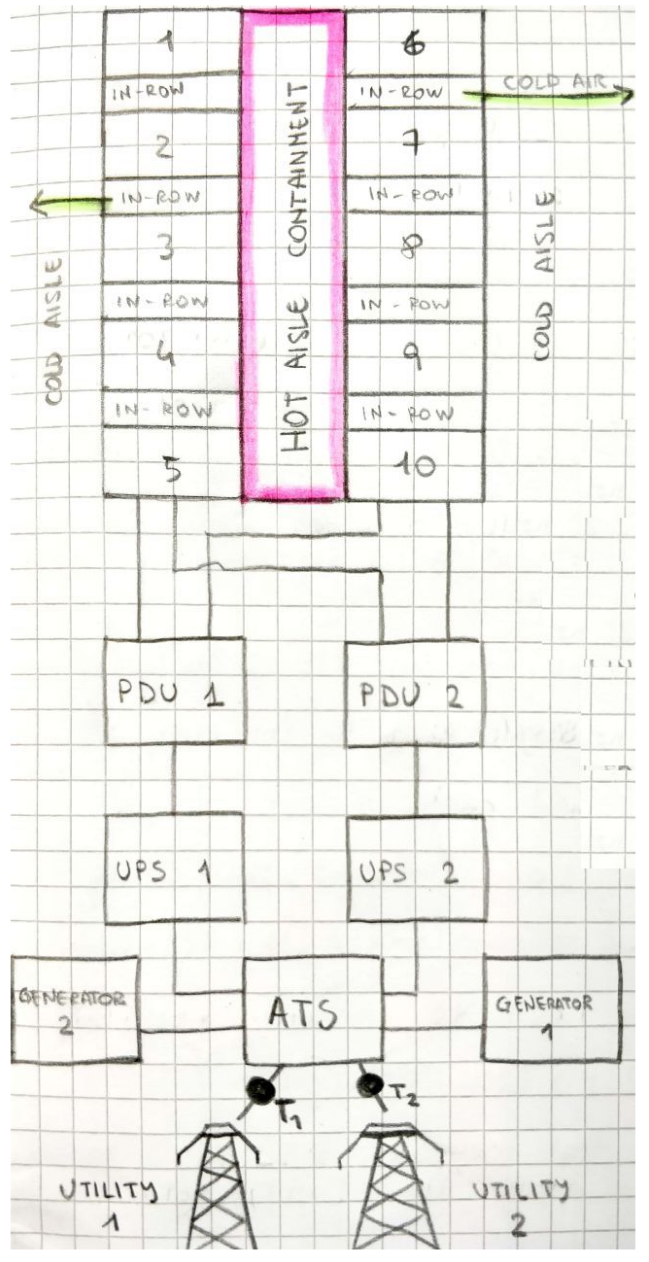
\includegraphics{images/datacenter_sketch.png}
    \caption{Solution 2 schema}
    \label{fig:10racks}
  \end{figure}
\end{paracol}

\hypertarget{san-vs-hyperconverged-architecture}{%
\section{4) SAN VS hyperconverged
architecture}\label{san-vs-hyperconverged-architecture}}

\hypertarget{question-3}{%
\subsection{Question}\label{question-3}}

A service requires a sustained throughput towards the storage of 15
GB/s. Would you recomment using a SAN architecture or a hyperconverged
one.

\hypertarget{solution-3}{%
\subsection{Solution}\label{solution-3}}

\begin{itemize}
\item
  15 GB is the max bandwidth of a PCI express bus with 16 lanes.
\item
  100 Gbps bandwidth of a single \textred{---FC?---} link (even if internally is 4*25 Gbps).
\item
  15 GBps * 8 = 120 Gbps
\item
  The PCI has some overhead, so it's bandwidth is not fully 15 GB.
\item
  15 GB = 54 TB/hour = 1 PB/day = half exaB / year. I have also to
  consider where am Is going to store this data, not focusing only on
  the bandwidth.
\item
  8/ 10 TB mechanical drive capacity.
\item
  SATA SSD has 500 MB bandwidth.\\
  \textred{What about NVMe?}
\item
  With 15 GB/sec, 4 fibre channel are enough.
\end{itemize}

\textbf{SAN area network (recap)}\\
SCSI internet protocol (SCSI on fiber) allows to mount blocks/disks.\\
Block-based access: you mount a chunk of bytes seen as a drive.\\
LUN (Logical UNits), can be replicated, compression can be used, it can
be overbooked.\\
Servers and drives are separated, drives are pooled togheter.

SAN today is failing because the bandwidth of the drives saturates the
links, making it impossible to pool a lot of drives.

\textbf{NAS}\\
It uses istead a network file system protocol to access the pooled
resources (SIFS, NFS). We access files not blocks.\\
NAS gives the file system, with SAN I decide the FS.\\
Security in SAN is bounded to the compute OS, which decide the
authentication domain.\\
Instead NAS has the responsibility of the security and the filesystem
abstraction(Active Directory and NFS security).

Both SAN and NAS separate the storage from the compute. Configure one
for all the storage (backup, compression\ldots) and look at it as blocks
or files.\\
This architecture is failing because of the throughput of the drive
(very fast) that saturates the link.

\textbf{HCI (hyperconverged)}\\
Before we talked about three independent units: compute, storage and
network. With HCI instead we have boxes (servers) with a little bit of
network, drive and compute.

It's not true that the compute and the drive are completely unrelated
and can be completely separated: also the CPUs have their own limits in
data processing even if large (risk to waste resources).

HCI by Nutanix allows to simply add a bit of storage, a bit of compute
and a bit of network by buying a server. You pay as you grow and lower
the risk, since you don't have to make capacity planning.

\textbf{Discussion}\\
The choice depends also on the kind of data I assume to process (assume
at least one: sensors, bank financial data \ldots). For example HCI is
not convenient if a want to do archiving because I pay for extra unused
CPU.

It's not enough to say: I take 5 big drives, because their bandwidth can
be a bottleneck.

SAN could be the good solution because it's cheaper. SAN can be used
with \textbf{tiering}: in the first layer I keep SSD ``buffers'', in the
second layer mechanical drives. If I keep a buffer of 1TB I'll have 6
minutes to copy down the buffered data to the mech drives.\\
Assuming 24 Gbps of incoming bandwidth and 1 TB of SSD buffer.\\
\textred{This way you would need 30 ($=\frac{15 GB/s}{500MB/s}$) SSD drives to avoid bottlenecking the incoming 15GBps bandwidth.}\\
24 Gbps = 3 GBps --\textgreater{} 1000 Gb /3 = 330 s to saturate the
buffer.\\
Netxt to the buffer there are mech drives (130/150 MBps)\\
I write to the SSD 3000 MBps but I copy to the drive (assuming just 1)
150 MBps. So the incoming bandwidth in the buffer is 3000 -150 = 2850
MB/s.\\
With one mech drive I will saturate the disk in 1000 GB / 2.8 GBps = 360
s = 6 min

If I consider the text of the exercise, in particular `towards', as in
the sense of ``only writing'', imagining to have to almost only archive
data and read only from time to time, I can actually consider SAN,
because if I go hyperconverged I am paying also for the CPU which might
be unused. If I instead have a balance between r/w and want a good
throughput for both operations, or I have a peek and then a flatter
period of time with few action, then I might choose better going
hyperconverged.

\textbf{What should I look for..}

\begin{itemize}
\item
  Capex Opex
\item
  Resilience
\item
  Bandwidth (network, drives)
\item
  etc\ldots{}
\end{itemize}

\hypertarget{dimension-a-hyperconverged-system}{%
\section{5) Dimension a hyperconverged
system}\label{dimension-a-hyperconverged-system}}

\hypertarget{question-4}{%
\subsection{Question}\label{question-4}}

A service requires a sustained throughput towards the storage of 15
GB/s. How would you dimension an hyperconverged system to ensure it
works properly?

\hypertarget{solution-4}{%
\subsection{Solution}\label{solution-4}}

Look first at the network (fabric is the glue of the infrastructure).
Can't have 100 GBps straight to the server because of spine and leaf, so
I have to consider the idea of distribution (hyperconverged).
\textred{Why not? 100Gbps is the max bandwidth of a single link, but we can have multiple links, right? Could I add more links/NICs?}

{\ns Recap that:
\begin{itemize}
\item
  just 1 or 2 ports of 100Gbps are enough to saturate the PCIe.
\item
  not good to have 100Gbps for each node cause I'm overloading that
  single node while HCI is distributed
\end{itemize}}

First I have to choose the Ethernet bandwidth between
(10-25-50-100-400), considering that 400 Gbps is achievable only on the
spine, and not on the leaves.\\
Better 10 Gbps or 25Gbps depending on CAPEX.\\
With spine and leaf I have 50 Gbps cause I double (active-active).

\textbf{Some calculations}\\
We have 15 GB/s incoming bandwidth --\textgreater{} 15 * 8 = 120 Gbps\\
We first dimension a spine and leaf architecture to sustain this
bandwidth value.\\
We have a couple of options:

\begin{itemize}
\item
  10 Gbps per server (hyperconverged node)
\item
  25 Gbps per server (we choose this)
\end{itemize}

To cover 120 Gbps we need at least 5 nodes --\textgreater{} 5*25 = 125
Gbps

We could also add more (up to 8-10) nodes to have redundancy and
efficiency, but we will consider 5 in the calculations

Every HCI node will have some SSD (as buffer) and some mechanical
drives.

Since we have 120 Gbps totally each node will receive 120 / 5 = 24 Gbps
storage bandwidth\\
This is ok since the link to the node is 25Gbps (even if we have
active-active configuration so the actual bandwidth is 50 Gbps)

Now we must consider the number of drives in each node. The drive
throughput must sustain the incoming bandwidth of 24Gbps to avoid data
loss. We know that SSD drives have a bandwidth of 500 MBps, so half a
GB.\\
So 24 Gbps / 8 = 3 GBps

\begin{itemize}
\item
  $\#disks \cdot (\dfrac{1}{2} GBps) = 3 GBps \Longrightarrow \#disks = 6$
\end{itemize}

Remember that bandwidth is not fully used because of some
overhead (e.g. to connect two spine nodes together).

\textred{So we have 5 leaf switches, each providing 25Gbps to the server, and each server has 6 disks, each providing 500MBps.\\
Using 5 servers we have 125Gbps of storage bandwidth, which is enough to sustain the 120Gbps of incoming bandwidth.\\
What has to be done at the spine layer? Which type of protocols and connectors must be used in order to achieve the abovementioned bandwidth?}

\hypertarget{other-questions}{%
\section{Other questions}\label{other-questions}}

\hypertarget{megantosh}{%
\section{@megantosh}\label{megantosh}}

My exam was a variation of the above questions:

\textbf{Design a data center that should contain 40 Racks, consuming 15
kW each. Discuss all necessary considerations, e.g.~Power Distribution,
Cabling, Cooling.}

drawing a scheme with the components like PDU etc. was appreciated.
Discussing firefighting, cooling using natural resources (water from
ocean etc.). Show that you can do the Math: 15000 Watt = 380 V * A * cos
fi where cos fi is the heat dissemination happening from conversion of
AC into DC current

\textbf{1024 Servers need to be connected with any of the following
switch options: 48x25Gbps East/West Traffic with 6 x 100 Gbps for
North/South (and two other configs to choose from). Oversubcription
level can be up to 1/6. Which network Topology would you choose? Discuss
its pros and cons.}

\hypertarget{solution-1-1}{%
\subsection{Solution 1}\label{solution-1-1}}

I gave a couple but he was more interested to see one discussed in
through detail. So not to recite theory but to be able to apply the
knowledge from the section above.\\
For 1024, 48x25, oversubscr 1/6. I went for spine/leaf model and he
wanted to know how many switches would be required in that case (do not
forget redudancy causes doubling + two links of the 6 will be gone for
connecting the two spines together)

\hypertarget{solution-2-2}{%
\subsection{Solution 2}\label{solution-2-2}}

E/W : 48 x 25 = 1200 Gbps

N/S : 6 x 100 = 600 Gbps

1200 / 600 = 2:1 Oversubcription (Good) \textred{Why is this good?}

How many switches should I buy?

1024/48 = 21,333 = 22 switches (leaves) at least \textred{Why 22? I don't get the math here. Are we dividing the number of servers by the number of ports?}

I don't have enough space to put every switch in a single rack (tor),
can I re-organize the infrastructure in order to save space?
\textred{What's tor? What's the advantage of putting switches in a tor?}

Yes, you can ``merge'' two switches phisically by switch aggregation and
put them in a rack (tor). To aggregate two switches, we need to connect
them with 2 cables (for resiliency). This means that we lost 2 ports on
each side, so, a new oversubcription ratio should be computed.

If we imagine two of the given switches put together, we get:

E/W : (2 x 48 ports) x 25 Gbps = 96 ports x 25 Gbps = 2400 Gbps

N/S : {[}2 x (6 - 2) ports{]} x 100 Gbps = 8 ports x 100 Gbps = 800 Gbps

2400 / 680 = 3:1 Oversubcription (Still good)

\textbf{How does live migration of a VM happen and would you prefer to
do it over HCI or SAN?}

as long as no detail is provided, you are allowed to make your own
assumptions.\\
I said both should be effectively the same given that bandwidth would
not be blocked and that we are using latest/fastest technology. Crucial
part of the VM Migration was (apart from copying config files, moving
virtual registers and halting the old machine for a millisecond) is that
copying the files happens in the background. If a file is required to
complete a process and it has still not been migrated, the new VM goes
and fetches it first from the old VM before it continues with copying
any other file*\\
\textred{Wasn't this related to (RAM) memory areas more than ``files''? Having a SAN allows to have a shared storage, so the VM can access the same data from both the old and the new machine. What about HCI? Should happen the same but inside the HCI ``box'', right?}

\textbf{Discuss the role (functions) of the orchestration layer. Give an
example workflow. where does it lie in the cloud stack?}

check the slides for sure, they are very helpful! A process I gave was
provisioning an Alexa skill on AWS which requires building a Lambda
function (an AWS service) and a Skill controller. I think he was happy
to have a real-life example. Draw the workflow like a business process
from the point of provisioning to the billing etc.

\hypertarget{giacomodeliberali}{%
\section{@giacomodeliberali}\label{giacomodeliberali}}

\textbf{What is a virtual firewall? Where will you put it? And how
many?}

TODO: answer

\textred{\textit{``Virtual''} firewall? Don't remember talking about that. However i would put one for each N/S link, probably none for E/W links, IDS/IPS there would be more appropriate, to detect lateral movements.}

\section{My exam session}
\subsection{Datacenter and Business informatics exams}

\begin{enumerate}
  \item What is PUE? How can you improve it? (...) Let's start from the definition. (...) What do you mean by ``apparent current''
  \item What is CRAC cooling? How is it different from InRow cooling?
  \item What is LACP?
  \item Difference between VMs and containers?
\end{enumerate}

\begin{enumerate}
  \item Network difference between container and vm
  \item Having solar panels would affect the PUE?
  \item Should you care about the PUE if you have solar panels?
  \item You have a system that generates 1 TB/s. Design system accordingly
  \item How would you design a fibre channel SAN with 100Gb/s input
  \item Would VM replicas affect SLA?
\end{enumerate}